%!TEX TS-program = xelatex  
%!TEX encoding = UTF-8 Unicode  

\documentclass[12pt]{article}  
\usepackage{geometry}  
\geometry{letterpaper}  
\usepackage{fancyhdr}
\usepackage{extramarks}
\usepackage{amsmath}
\usepackage{amsthm}
\usepackage{amsfonts}
\usepackage{tikz}
\usepackage[plain]{algorithm}
\usepackage{algpseudocode} 
\usepackage{caption}
\usepackage{booktabs}
\usepackage{graphics}
\usepackage{amsmath}
\usepackage{amsfonts}

\usepackage{xltxtra,fontspec,xunicode}
\usepackage[slantfont,boldfont]{xeCJK}
\setCJKmainfont{宋体}   
\setmainfont{Optima}   
\defaultfontfeatures{Mapping=tex-text}  

\usepackage{xltxtra,fontspec,xunicode}
\usepackage[slantfont,boldfont]{xeCJK}
\setCJKmainfont{宋体}   
\setmainfont{Optima}   
\defaultfontfeatures{Mapping=tex-text}  

\XeTeXlinebreaklocale “zh”  
\XeTeXlinebreakskip = 0pt plus 1pt minus 0.1pt   
 
\usepackage{listings}
\usepackage{color}
\definecolor{dkgreen}{rgb}{0,0.6,0}
\definecolor{gray}{rgb}{0.5,0.5,0.5}
\definecolor{mauve}{rgb}{0.58,0,0.82}

\lstset{frame=tb,
  language=Java,
  aboveskip=3mm,
  belowskip=3mm,
  showstringspaces=false,
  columns=flexible,
  basicstyle={\small\ttfamily},
  numbers=none,
  numberstyle=\tiny\color{gray},
  keywordstyle=\color{blue},
  commentstyle=\color{dkgreen},
  stringstyle=\color{mauve},
  breaklines=true,
  breakatwhitespace=true,
  tabsize=3
} 

\topmargin=-0.45in
\evensidemargin=0in
\oddsidemargin=0in
\textwidth=6.5in
\textheight=9.0in
\headsep=0.25in

\linespread{1.1}

\pagestyle{fancy}
\lhead{\hmwkAuthorName}
\rhead{\hmwkClass}
\chead{\hmwkTitle}

\renewcommand\headrulewidth{0.4pt}
\renewcommand\footrulewidth{0.4pt}

\setlength\parindent{0pt}

% Homework Details

\newcommand{\hmwkTitle}{homework\ \#4}
\newcommand{\hmwkClass}{Deep Reinforcement Learning}
\newcommand{\hmwkAuthorName}{Tianxiao Hu}


\begin{document}
\pagebreak

\section{Problem 1}
\begin{figure}[!h]
\centering
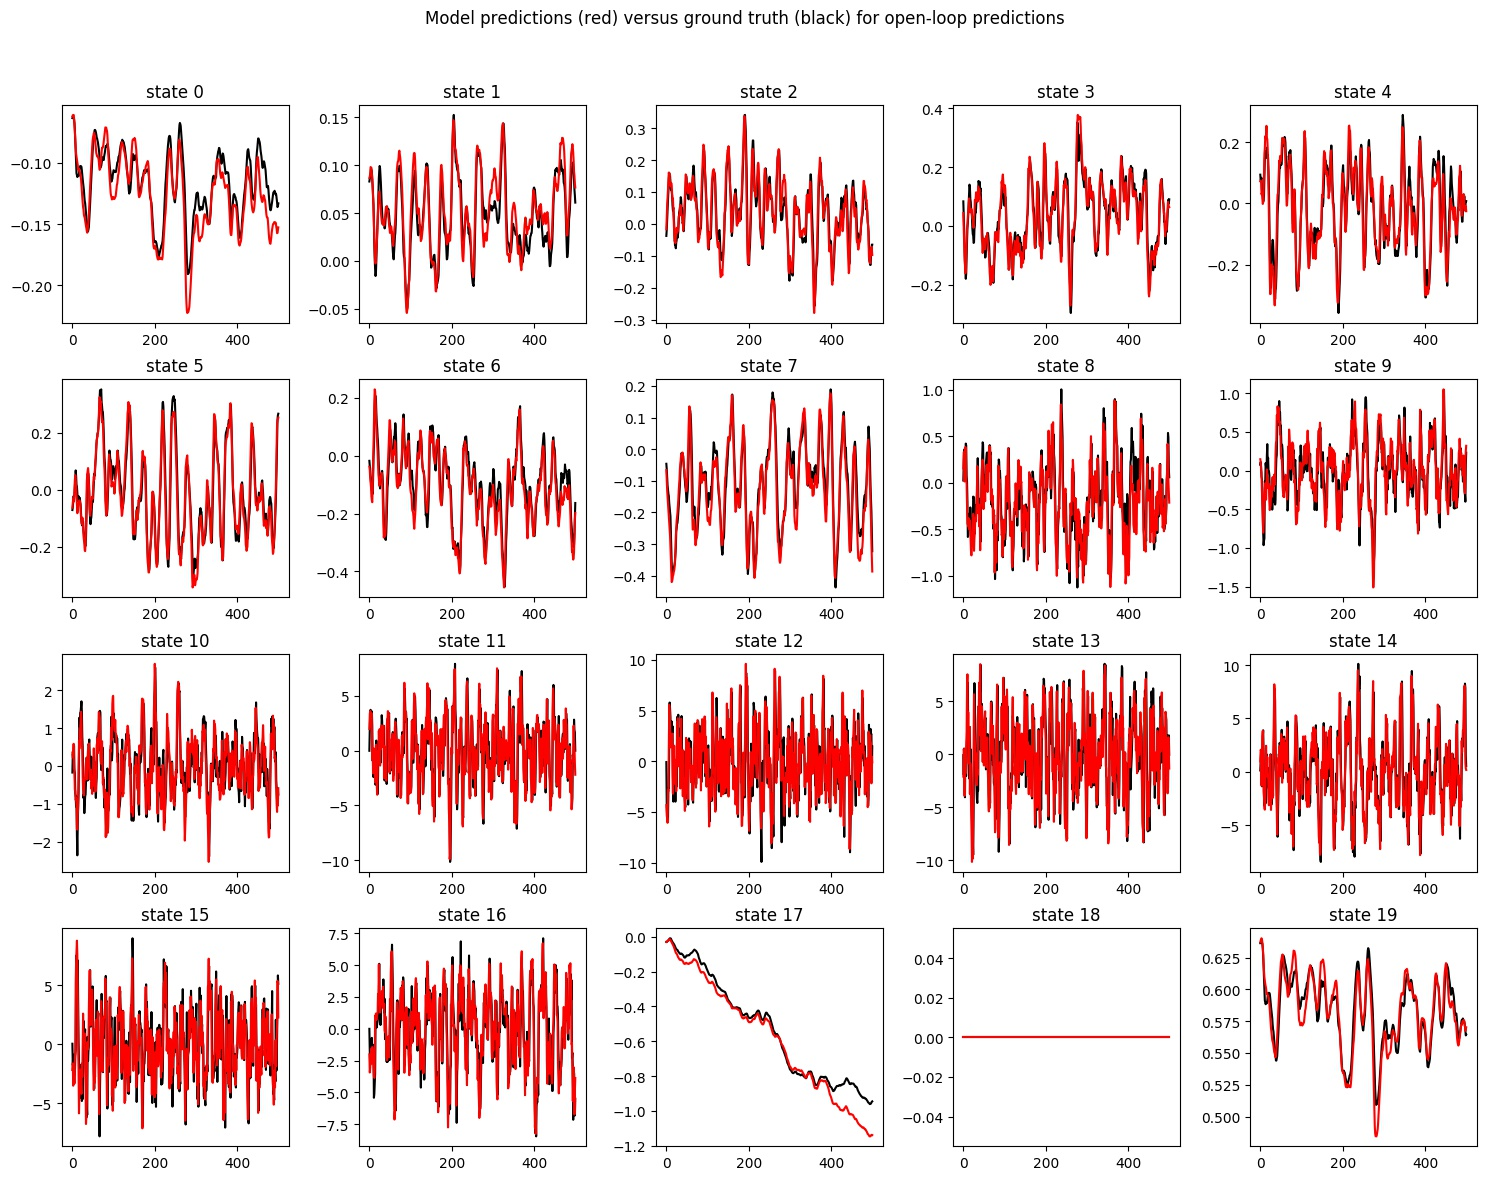
\includegraphics[width=5in]{Figure_1.jpg}
\caption{Performance for best model with most accurate predictions.}
\end{figure}

State 17 is most inaccurate prediction among all states. For the early prediction error will accumulate and affect the later prediction. In other words, small errors can add up to large ones.

\newpage
\section{Problem 2}

\begin{table}[!h]
\begin{center}
\begin{tabular}{@{}l|l|l@{}}
\toprule
          & random policy & model-based policy \\ \midrule
ReturnAvg & -170.73 & 23.25                 \\
ReturnStd & 91.32   & 22.35                 \\ \bottomrule
\end{tabular}
\caption{{\em ReturnAvg} and {\em ReturnStd} for random policy and model-based policy.}
\end{center}
\end{table}

\newpage
\section{Problem 3}
\begin{figure}[!h]
\centering
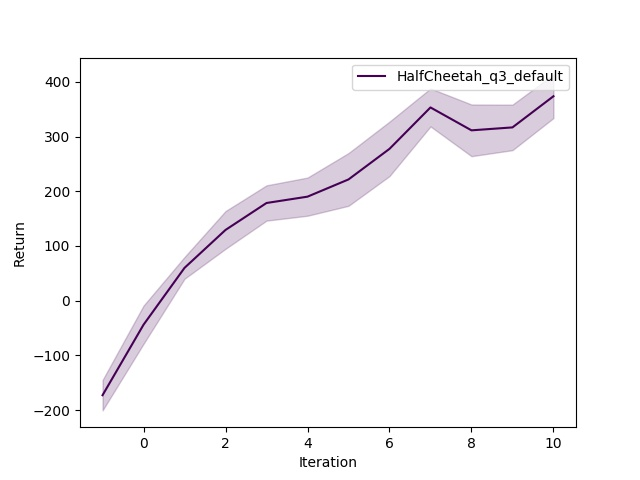
\includegraphics[width=5in]{Figure_2.jpg}
\caption{Returns versus iteration when running model-based reinforcement learning.}
\end{figure}

\newpage
\section{Problem 4}

\begin{figure}[!h]
\centering
\begin{minipage}[t]{0.48\textwidth}
\centering
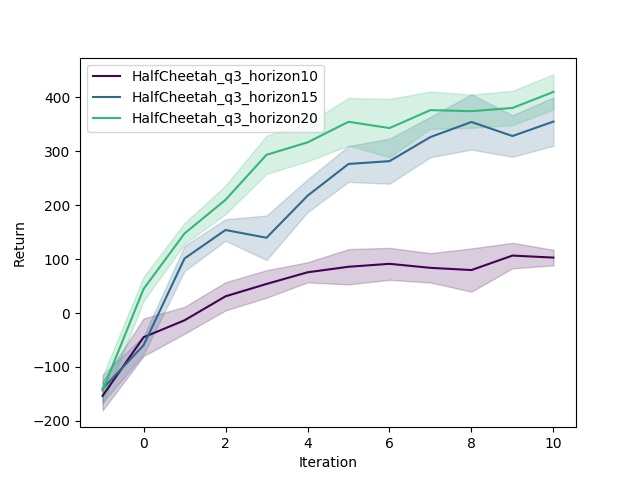
\includegraphics[width=8cm]{Figure_3.jpg}
\caption{Model performance with different MPC horizon.}
\end{minipage}
\begin{minipage}[t]{0.48\textwidth}
\centering
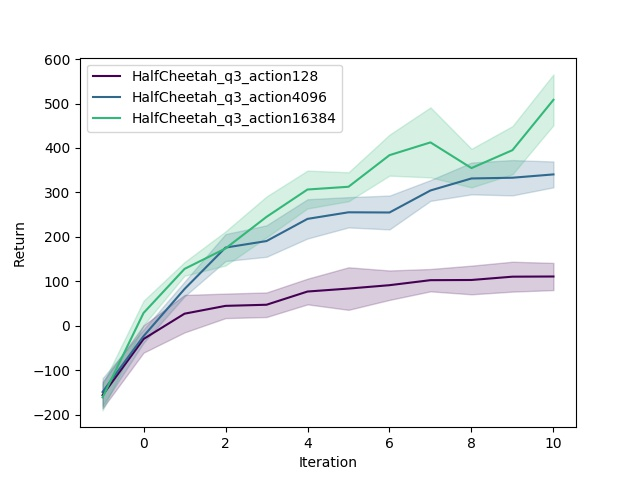
\includegraphics[width=8cm]{Figure_4.jpg}
\caption{Model performance with different number of randomly sampled action sequences.}
\end{minipage}
\end{figure}

\begin{figure}[!h]
\centering
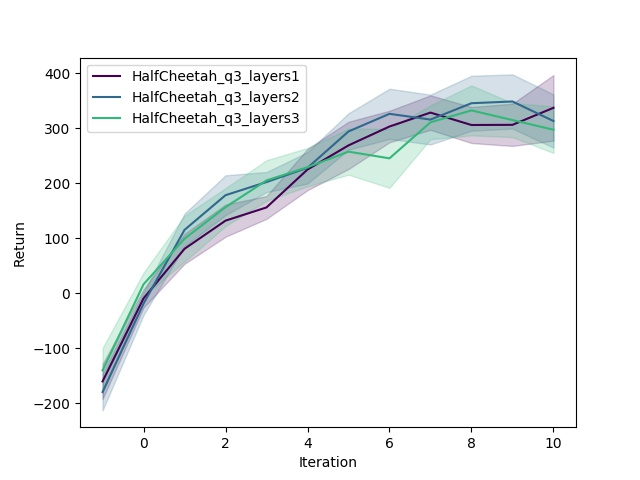
\includegraphics[width=3.3in]{Figure_5.jpg}
\caption{Model performance with different number of neural network
layers.}
\end{figure}

\end{document}  
  